\chapter{Software architecture and Methodology}
\noindent This chapter provides the details of the software architecture and the methodology of Modulo7 and also lists the limitations of the Modulo7 software implementation. 
\section{Server Side architecture}
\noindent Modulo7 is designed with the purpose of scalability. Modulo7 is built up of the following modules
\begin{enumerate}
\item \textbf{Source Converters} : Converts music sources (e.g. music XML, midi etc) into Modulo7's binary representation.
\item \textbf{Music Theory Models} : These models are implementations of the music  theoretic criteria formalized in \ref{similarity}, \ref{statistic} and \ref{criteria} as well as the vector space models defined in \ref{polyphonicvectors}
\item \textbf{Persistent Storage Mechanism} : The Modulo7 internal representation is implemented as a hierarchical class design as shown in \ref{fig:figureDocStruct}. This representation is then serialized via Apache Avro \ref{avro} and stored to disk. 
\item \textbf{Lyrics Indexer} : An inverted index of song lyrics. This acts as a base on which standard techniques for similarity analysis might be applied. Alternatively it can provide a framework on which custom models (e.g. semantic intent of the song, correlation between music theory models and lyrics) might also be applied. Apache Lucene was used for developing the document index for lyrics \ref{lucene} and alchemy \ref{Alchemy} was used semantic intent and language ID feature implementations.  
\item \textbf{Lyrics similarity models} : A set of similarity models that can be applied to indexed lyrics objects. Modulo7 also implements meta data predictor models described in \ref{lyricsarch}. 
\item \textbf{Query Engine} : An SQL like interface to a client that allows you to gather and ascertain useful information (based on music theoretic criteria). Antlr was used for developing a lexer and parser for this engine \ref{antlr}. 
\end{enumerate}

\begin{figure}
\centering
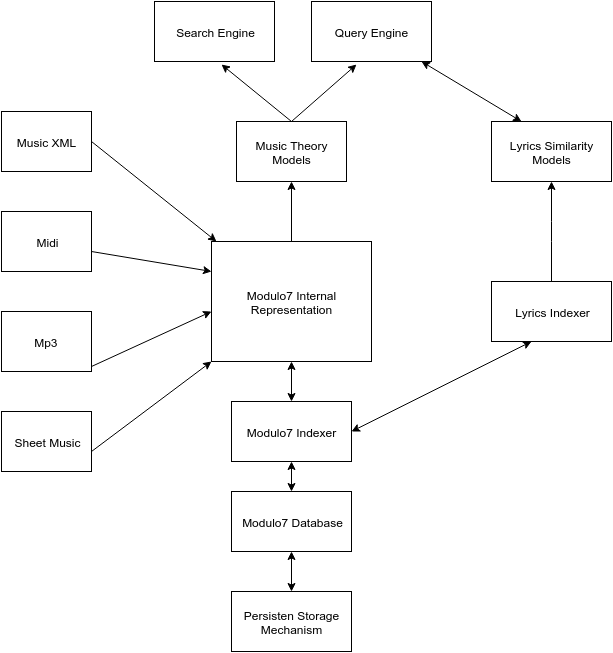
\includegraphics[width=\textwidth]{Modulo7Architecture.png}
\makeatletter
\let\@currsize\normalsize
\caption{Block diagram of Modulo7 software architecture}
\label{fig:Architectural Design}
\end{figure}
\newpage
\section{Client architecture}
\noindent The server exposes a sql like interface with a query syntax defined in \ref{m7sql} and a standard querying set defined in \ref{standardquery}. \\

\noindent Moreover the client also exposes a highly customized search engine based on the vector space representations defined in\ref{polyphonicvectors}. The search engine implements the ranked order search based on the similarity measures defined in \ref{similarity}. 

\section{Song sources and Parsers} \label{m7songsources}
\noindent At the heart of Modulo7's design is its song sources parsers (or converters) which converts different song sources into its own internal binary format \ref{fig:figureDocStruct}. Each music source is a different representation and while certain sources ascribe what how music should be played (e.g music-xml, sheet music), other formats ascribe what is actually being played (e.g midi, mp3). There are many other music sources in existence (e.g guitar tablature, GUIDO format , humdrum kern format \ref{musicrepresentation} etc), but for the purposes of breadth and ubiquity, four sources have been targeted as input for Modulo7(mp3, sheet music as png, jpeg etc, music xml file and midi files). Its important to note that acquiring features from each format is a domain specific challenge and inaccuracies are inherent because of that. Moreover Modulo7 does not attempt to improve on state of the art feature extraction techniques. The following subsections describe the individual formats in detail and the challenges encountered in parsing them.

\subsection{Midi format}
\noindent MIDI (short for Musical Instrument Digital Interface, is a technical specification for encoding of events on a midi enabled instrument and a protocol for interfacing and communicating between various midi enabled instruments \cite{midispec}. Typically any midi enabled electronic instrument when played, relays to its internal circuitry a message. Examples of such messages could be a particular note is being hit on a keyboard, a note is being hit off after being hit on, tempo based messages on the number of ticks per second etc. While MIDI is a technical specification for encoding music the score is being played, Modulo7 treats it as a symbolic representation of music. Midi was also a simple and popular encoding format for music and gaming industry in the  1990s. \\

\noindent Midi is one of the easier formats to parse for symbolical music information. Moreover there is a big volunteer community of midi encoders. As such acquiring and parsing non trivial amounts of midi data is not a very challenging task. 

\subsection{Western Digitized Sheet Music} \label{digitizedsheet}
\noindent Sheet music is one of the oldest forms of music in existence. Its a hand written or printed form of music that uses a specific script (a set of musical symbols on a manuscript paper) to ascribe music. Music Composers from Medieval and Modern periods of the western world use western sheet scripting to codify their work while performers play from these sources. A vast body of older work and particularly orchestral work is codified in sheet music \cite{theorytreatise}. \\

\noindent Like midi, sheet music is also symbolic in nature. However unlike midi, its an expression of how a score should be played, rather than what is being played. Modulo7 converts digitized versions of these sheet music (e.g sheet music stored .tiff, .png. jpeg etc formats). \\

\begin{figure}
\centering
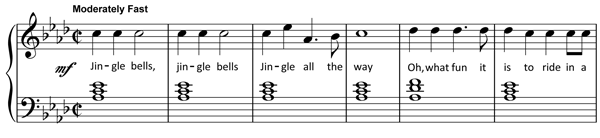
\includegraphics[width=\textwidth]{jingle-bells-sheet-music-piano.png}
\makeatletter
\let\@currsize\normalsize
\caption{Jingle bells melody sheet music representation}
\label{fig:sheetmusicexample}
\end{figure}

\noindent Parsing digitized sheet music is an extremely challenging task. It requires a solid understanding of computer vision algorithms and even the state of the art software in existence today cant handle all scores (especially for poorly digitized formats \cite{gamera}). Given the amount of domain knowledge required, Modulo7 uses a third party library called Audiveris \ref{audiveris} for the purposes of Optical Music Recognition. 

\subsection{Music XML format}
\noindent Music XML format is an xml based standard open format for exchanging digital symbolic music \cite{musicxmlspecification}. A music XML format is unusual as its a format that is easy to parse for computers and easy for humans to understand it. MusicXML formats are heavily used by music notation applications. Music XML format is a symbolic format and can be considered a modernization of the Sheet music format. Its disadvantage however is unlike sheet music, a performer cant read the piece and play it on the spot directly. \\

\noindent Just like Western Sheet music and midi, music XML is a symbolic format as well. Music XML is also a transcription format which specifies how a score should be played. 

\subsection{MP3 format} \label{mp3format}
\noindent For the sake of completeness, Modulo7 also supports an audio format called mp3. Its an audio encoding format that uses lossy compression to encode audio data \cite{mp3specification}. Mp3 gives a reasonably good approximation to other digital audio formats of music storage with a significant savings in space for storage. Its one of the de-facto standards of digital music compression and transfer and playback on most digital audio players. In order to parse this format, Modulo7 uses the technique developed in \ref{chromagramest} and also utilizes the Echo Nest jEN API for directly processing mp3 files into chromagrams \ref{echonestjen}. 

\section{Modulo7 Internal Representation}

\noindent Modulo7 consists of converters that convert data into Modulo7's internal representation \ref{m7songsources}. This representation can be thought of a document representation on which similarity measures described in \ref{similarity} can be applied on. Moreover the internal representation can be thought of as an indexed meta data structure for any source of song from which relevant information can be acquired. Hence Modulo7 indexing schematic is a symbolic representation of music similar to the music xml and sheet music formats. Its important to note that depending on there source one or more of the subcomponents of the internal representation may be missing or wrong. Modulo7 indexes songs based on certain criteria and on top of these boolean queries can be formulated. The internal components are categorized as the following:-\\

\noindent \textbf{Song Metadata:} The meta data aspects of a song e.g. The name of the song/ the composer/performer's name, Key Signature of the Song, Meter of the Song etc. These are global properties of a particular song. \\

\noindent \textbf{Voices in a song:} An implementation of the voices described in \ref{voice}, voices in Modulo7 represent the same symbolic data as is present in the sources from which the information is parsed.\\

\noindent \textbf{Lyrics of a song:} The textual representation (along with delimiters for line breaks) for the lyrics of a song. Lyrics can live independently as separate entities (if the input to Modulo7 is a text file containing the lyrics and no other information). However midi/musicxml and sheet music have optional lyrics elements present in their transcriptions and Modulo7 transcribes the lyrics from them. \\

\noindent In most cases though lyrics exists as a separate entity from songs. In such cases, Modulo7 separately indexes lyrics. In certain datasets, the lyrics representation is different (for example the million song dataset has a representation format as a bag of words with counts of the words occuring for each format \cite{msd}). Modulo7 accomodates such formats as well.

\begin{figure}
\centering
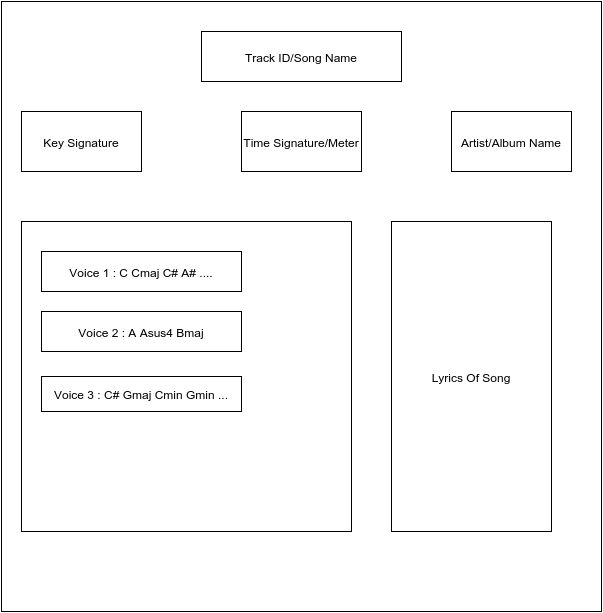
\includegraphics[width=\textwidth]{DocumentStructureOfModulo7.png}
\makeatletter
\let\@currsize\normalsize
\caption{Abstract representation of the Modulo7 internal representation}
\label{fig:figureDocStruct}
\end{figure}

\newpage

\section{Methodology}

\noindent This section contains the methodology followed in the information retrieval phase and then the indexing steps taken after the domain specific conversion is completed by Modulo7's adapters

\begin{enumerate}
\item Given a root directory, Modulo7 recursively parses all the sheet music image files, mp3, midi and music xml files. Depending on the file type individual parser modules are invoked and an internal representation is created in memory and serialized to disk (depending on user preference)
\item Modulo7 then indexes all the objects created on specific meta data (such as key signature, time signature and artist of a song). Moreover it also creates a lucene index on lyrics extracted. It stores all these indices in memory. 
\item Modulo7 then exposes a prompt to the consumer a standard query set \ref{standardquery}, or a customized structured query prompt \ref{m7sql} or a customized similarity based search engine \ref{simengine}. 
\end{enumerate}

\subsection{Modulo7 standard query set} \label{standardquery}

\noindent Modulo7 exposes a standard set of querying features to the consumer. These queries are useful to extract simple information from the parsed dataset from Modulo7. The following are some sample queries that can be relevant for a user

\begin{enumerate}
\item Return all songs that are in the key of CMajor
\item Return all songs that are in in the Minor scale
\item Return a ranked order of lyrics similar to an input string (for example a verse in the song). 
\item Return all songs that are performed by Led Zepplin
\item Return all polyphonic songs in the database
\end{enumerate}

\noindent The simple query framework has limited expressiveness in querying options but is an example set to the user on what can be queried. Modulo7 also exposes a more customized and expressive SQL like query syntax to concatenate boolean expressions of these example queries and more (boolean combinations of all criteria and statistics defined in criteria \ref{criteria} and statistic \ref{statistic} sections)

\subsection{Modulo7 SQL Language Specifications} \label{m7sql}

\noindent On top of the standard set of query set defined as an example set, Modulo7 also supports a custom query language for extracting relevant information from a parsed and indexed data set. This language is similar to SQL but its internal processing is radically different as it does not operate on a traditional database (it rather interacts with the Modulo7 indexer). A generic expression can be expressed as follows
\begin{equation}
\textbf{select input\_src\_list  from DATABASENAME where expr\_list}
\end{equation}

\begin{enumerate}
\item \textbf{input\_src\_list} : An argument list of all the acceptable formats of is any combination of songs : midi, musicxml, sheet and mp3. This de-selects out all the formats that are irrelevant to the consumer. 

\item \textbf{DATABASENAME} : The name of the Modulo7 Database. Its acts as an internal consistency check to determine if the consumer is querying against the right Modulo7 database. 

\item \textbf{expr\_list} : A conjunctive and/or disjunctive list of boolean queries on statistics and criteria defined in sections \ref{criteria} and \ref{statistic}. This allows for a greater degree of customization as compared to the other frameworks in literature as well as expose a structured query language for querying (which is sorely lacking in other frameworks). The elements of the expr\_list are defined as follows:-

\begin{enumerate}
\item \textbf{criteria is or is not true} : Returns a subset of songs from a candidate set which either satisfy or do not satisfy a given criteria. The argument criteria is replaced by an implemented criteria in \ref{criteria}
\item \textbf{statistic relational\_op doubleValue} : Returns a subset of a songs from candidate set which satisfy this criteria : When a statistic is applied on a song in a candidate set, the returned value of the statistic satisfies a relation a given value defined by the relational\_op argument. The arguments to this expression is a statistic implemented in \ref{statistic}, a relational operator and a double value.
\item \textbf{statistic between value1 and value2} : This form is a range query. This query returns the subset of songs from a candidate set which satisfy this criteria : When a statistic is applied on a song in a candidate set, the returned value lies in between value1 and value2. 
\end{enumerate}
\end{enumerate}

\noindent Each of these basic query component returns a subset of songs that satisfy the query component. These query components can be concatenated conjunctively or disjunctively to form a boolean query. So a query is effectively $Q = \cup_i | \cap_i (qc)$, where qc is a query component described above and Q is the resultant query. 

\subsection{Modulo7 Similarity Engine} \label{simengine}

\noindent On top of Modulo 7 supporting custom queries, it also acts in a ranked search engine mode. However the ranking model of the search engine is based on similarity measures based on the structural analysis of the music sources and are described in \ref{similarity} and the songs themselves are represented as vector space models defined in \ref{polyphonicvectors}.  \\

\noindent The similarity engine functions by asking the user for a reference "query" song and a similarity measure implemented in \ref{polyphonicsim}. The engine computes the similarity of the query song to each song in the indexed databased and returns a ranked order based on relevance to that particular similarity measure. 

\subsection{Modulo7 Lyrics Analyzer Architecture} \label{lyricsarch}

\noindent The modulo indexer also indexes lyrics, but treats lyrics objects as standard text documents. So the standard model of text Information Retreival techniques can be used to directly analyze lyrics. Modulo7 implements lyrics indexing and standard NLP operations on lyrics.

\begin{enumerate}
\item Modulo7 parses lyrics components from some of its sources (for example musicxml and midi have embedded lyrics structures inside it). This is stored along with the song object
\item Modulo7 also parses independent lyrics structures provided to it. This allows for increased flexibility for Modulo7 to just parse lyrics objects
\item Modulo7 creates a Apache Lucene \ref{lucene} index of the lyrics objects once parsed from its sources. This allows for users to make standard text queries via Lucene. 

\end{enumerate}

\noindent Modulo7 also provides support for rudimentary Natural Language Processing operations on top of the lyrics obtained. Two supported operations for lyrics are :-

\begin{enumerate}
\item \textbf{Language ID} : Modulo7 can detect what language the song's lyrics is written in. It does this via an language ID call to alchemy \ref{Alchemy}. 
\item \textbf{Sentiment Analysis} : Modulo7 can detect the positivity or negativity sentiment of a song's lyrics and assigns a score to it (with -1 standing for highest degree of negativity and similarly 1 standing for highest degree of positivity). It does this via a sentiment analysis call to alchemy. \ref{Alchemy}
\end{enumerate}

\section{Lyrics Based Genre Estimation} \label{genreestimation}

\noindent On top of these features, the lyrics analyzer provides support for genres prediction. Given a data set with genre annotations to songs along with lyrics, Modulo7 can predict genre annotations for new input lyrics. The following genre estimation schemes are implemented in Modulo7:-

\subsection{Naive Genre Estimation} \label{NaiveGenre}

\noindent Consider $T(S_i)$ be defined as the set of genre annotations for the song $S_i$ which is the $i^{th}$ song in a tag annotated data set. Let $S_{new}$ be a new song for which genre annotations need to be predicted and let L(S) represent the lyrics of a song. Hence $L_{new}$ should be similar to some $L(S_k)$ for their genres to be deemed identical. Let $S_{sim} = \{S_i | \ \ isSim(S_i, S_{new}) \geq \epsilon\} $ be the set of all the songs similar to $S_{new}$(Here $\epsilon$ is some thresh hold value and isSim is a similarity function that compares lyrics of two songs). We define $T_{new} = \{\cup \ T(S_i) \ | \ S_i \in S_{sim}\}$. In other words the genres of the new song is the union of the genre labels in the songs similar to the new song up to a particular thresh hold.

\subsection{Weighted Genre Estimation} \label{WeightedGenre}

\noindent In the previous scheme, there are no considerations for degree of importance of each tag for a give lyrics or about the degree of similarity between lyrics. In order to accommodate these we assume the existence of tag weights associated for tags in the song meta data. Let $T(S_i)$ be defined as the weighted genre annotations for song $S_i$. Let $S_{sim} = sort_v^{desc}({S_i, | isSim(S_i, S_{new}) = v})$ be the rank ordered set of genre labels based on descending order of similarity values, where isSim may choose to leverage the weights of tags to compute similarity. Out of these top we choose the top k $S_{sim(k)} = first_{k} (S_{sim})$ similar songs. The genre estimation can then be defined as $T_{new} = \{\cup \ T(S_i) \ | \ S_i \in S_{sim(k)}\}$ \\\\
This scheme takes into account the rank of the songs in based on a similarity metric. The scheme can retain only a subset of the maximal weighted tags in the resulting tag set for the input song and the size of this subset depends on the chosen value of k. 

\subsection{Max Frequency Tag Estimation} \label{MaxFrequencyGenre}

\noindent In the previous scheme, the frequency of genre labels occurring inside the dataset is ignored. In order to accommodate that let $f_x(S_i)$ be the total frequency of genre label x for the set $S_{sim}$ where $S_{sim} = \{S_i | \ \ isSim(S_i, S_{new}) \geq \epsilon\}$ where isSim and $\epsilon$ is defined identically in \ref{NaiveGenre}.  Hence we can define the set of estimated tags as $T_{new} = first_{k} sort_{f_x(S_i)}(x)$ where k is defined identically in \ref{WeightedGenre}. The tags are sorted according to descending cumulative frequencies of tags in the similar set. 

\section{Meta data Estimation} \label{metadataestimation}

\noindent Unlike other frameworks, Modulo7 attempts to attempts to guess and fill certain meta data that are missing in song sources. One such meta data is key signature of a song which it guesses is the Key Signature of a song via the algorithm described in \ref{kktonality} 

\section{Limitations of Modulo7}  \label{limitations}

\noindent While Modulo7 attempts to solve a large set of problems, there are some fundamental limitations to what Modulo7 can or cannot do. Some of the notable ones are listed as follows:-

\begin{enumerate}
\item Modulo7 does not perform any kind of timbral analysis. This limitation is by design, since all formats of music do not convey timbral information faithfully (for instance sheet music is a specification of music to be played and not an actual recording), hence Modulo7 has not been designed with timbral analysis in mind.
\item Modulo7 does not take into account varying time and/or key signatures. This is due to the fact that in most western music, these two global parameters stay constant. Also Modulo7 does not take into account atonal music (as a key signature leads to transforms that are needed in certain similarity metrics \ref{sim:preprocess}). 
\item Modulo7 assumes input mp3 files are monophonic. This is due to the fact that the state of the art in audio processing techniques have not solved the problem of polyphonic symbolic transcription faithfully. \cite{melextract}
\end{enumerate}
